\documentclass{article}
\usepackage[utf8]{inputenc}
\usepackage{graphicx}
\usepackage{fancyhdr}
\usepackage{listings}
\usepackage{color}
\usepackage{hyperref}
\usepackage{amsmath}



\graphicspath{ {images/} }

\pagestyle{fancy}



\title{%
    An Introduction of High Performance Computing \\
    \vspace{0.4cm}
    \large Lecture Notes
}

\author{jerakrs}
\date{January 2018}


\begin{document}

\maketitle

\begin{abstract}
    This document is the lecture note of \textit{An Introduction of High Performance Computing}. The course code is \textit{COMS30005} and the unit director is \textit{Simon McIntosh-Smith}.
\end{abstract}


\section{BlueCrystal}

BlueCrystal is the University's High Performance Computing machine. BlueCrystal Phase 3 (\textit{bluecrystalp3.bris.ac.uk}), is available to all users. Phase 4 (\textit{bc4login.acrc.bris.ac.uk}) is primarily intended for large parallel jobs and for work requiring the Nvidia P100 GPUs.


\subsection{Logging In}

\indent BlueCrystal only allows the user who is inside the University firewall to access directly.

Logging in the BlueCrystal Phase 3 by ssh command:

\begin{lstlisting}[language=Bash]
    $ ssh username@bluecrystalp3.bris.ac.uk
\end{lstlisting}

Changing password, run this command and follow the prompts to type the old and new password:

\begin{lstlisting}[language=Bash]
    $ passwd
\end{lstlisting}

It can use graphical tools remotely by adding \textbf{-X} flag when connecting:

\begin{lstlisting}[language=Bash]
    $ ssh -X username@bluecrystalp3.bris.ac.uk
\end{lstlisting}

Passwordless access, it allows user to set up the SSH keys so that the user can connect BlueCrystal without typing password:

\begin{lstlisting}[language=Bash]
    $ ssh-copy-id username@bluecrystalp3.bris.ac.uk
\end{lstlisting}

\noindent This command will copy the content of the \textit{public key} file (\textbf{id\_rsa.pub}) to BlueCrystal's \textbf{$\sim$/.ssh/authorized\_key}. If there no SSH key in local machine, run this command to make a new key:

\begin{lstlisting}[language=Bash]
    $ ssh-keygen
\end{lstlisting}


\subsection{The Queuing System}

BlueCrystal Phase 3 is made up of 4 head nodes and 341 computing nodes. The user will work on the headnodes, but the tasks should run on the computing nodes. Therefore there is a queuing system to manage jobs.

\begin{figure}[h]
    \centering
    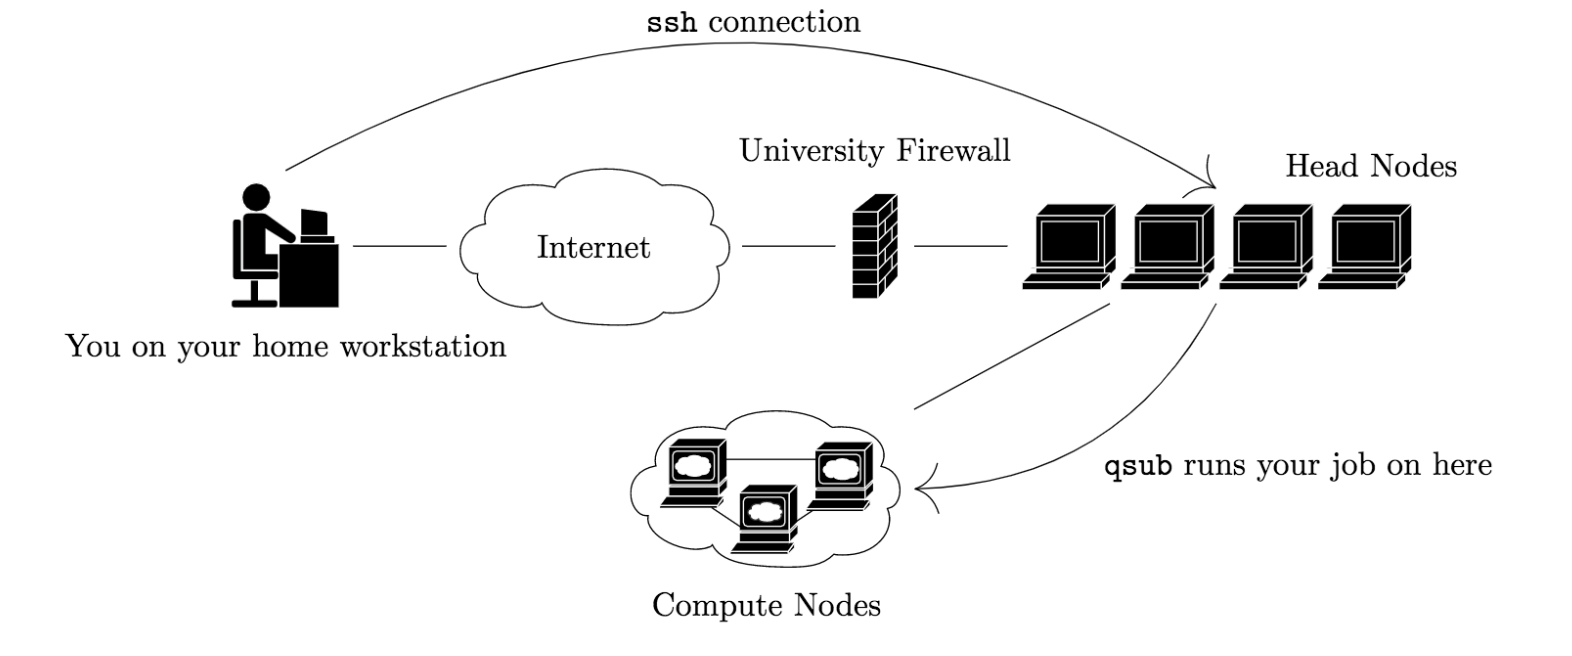
\includegraphics[scale=0.4]{images/structure-of-queue.png}
    \caption{The Structure of Queuing System}
    \label{fig:my_label}
\end{figure}

Submitting the jobs by qsub command:

\begin{lstlisting}[language=Bash]
    $ qsub example.job
\end{lstlisting}

\noindent The \textbf{example.job} is a script file, the content of this file is shown below.

\begin{lstlisting}[
    language=Bash,
    frame=shadowbox,
    numbers=left,
    caption=Example Script File]
#!/bin/bash

#PBS -N lab1
#PBS -o lab1.out
#PBS -joe
#PBS -q teaching
#PBS -l nodes=1:ppn=16
#PBS -l walltime=00:01:00

cd $PBS_O_WORKDIR

echo Running on host `hostname`
echo Time is `date`
echo Directory is `pwd`
echo PBS job ID is $PBS_JOBID

./lab1
\end{lstlisting}

Viewing the status of submitted jobs:

\begin{lstlisting}[language=Bash]
    $ qstat -u $USER
\end{lstlisting}

\noindent The S column gives the job status. \textbf{R = running, C = complete, Q = queued}.

Deletingthe a submitted job:

\begin{lstlisting}[language=Bash]
    $ qdel jobid
\end{lstlisting}


\subsection{Environment Modules}

BlueCrystal has lots of extra software, it allows users to load the modules which they need. When user submits a new job, it need to load the modules that this task will use in the script file, or put them into the user's \textbf{.bashrc} file so they are loaded when user log in and for every job the user run.

View available software:

\begin{lstlisting}[language=Bash]
    $ module avail
\end{lstlisting}

Combining the grep command, it can search the module:

\begin{lstlisting}
    $ module avail 2>&1 | grep intel
\end{lstlisting}


Load and unload the module:

\begin{lstlisting}[language=Bash]
    $ module load languages/gcc-4.8.4
    $ module unload languages/gcc-4.8.4
\end{lstlisting}

List loaded modules:

\begin{lstlisting}[language=Bash]
    $ module list
\end{lstlisting}


\section{Processors}

The most important HPC trends:

\begin{itemize}
    \item Microprocessor performance $\sim55\%$ per annum.
    \item Memory capacity $\sim49\%$ per annum.
    \item Memory bandwidth $\sim30\%$ per annum.
    \item Memory latency $<< 30\%$ per annum.
\end{itemize}


Cache Hierarchy:

\begin{figure}[h]
    \centering
    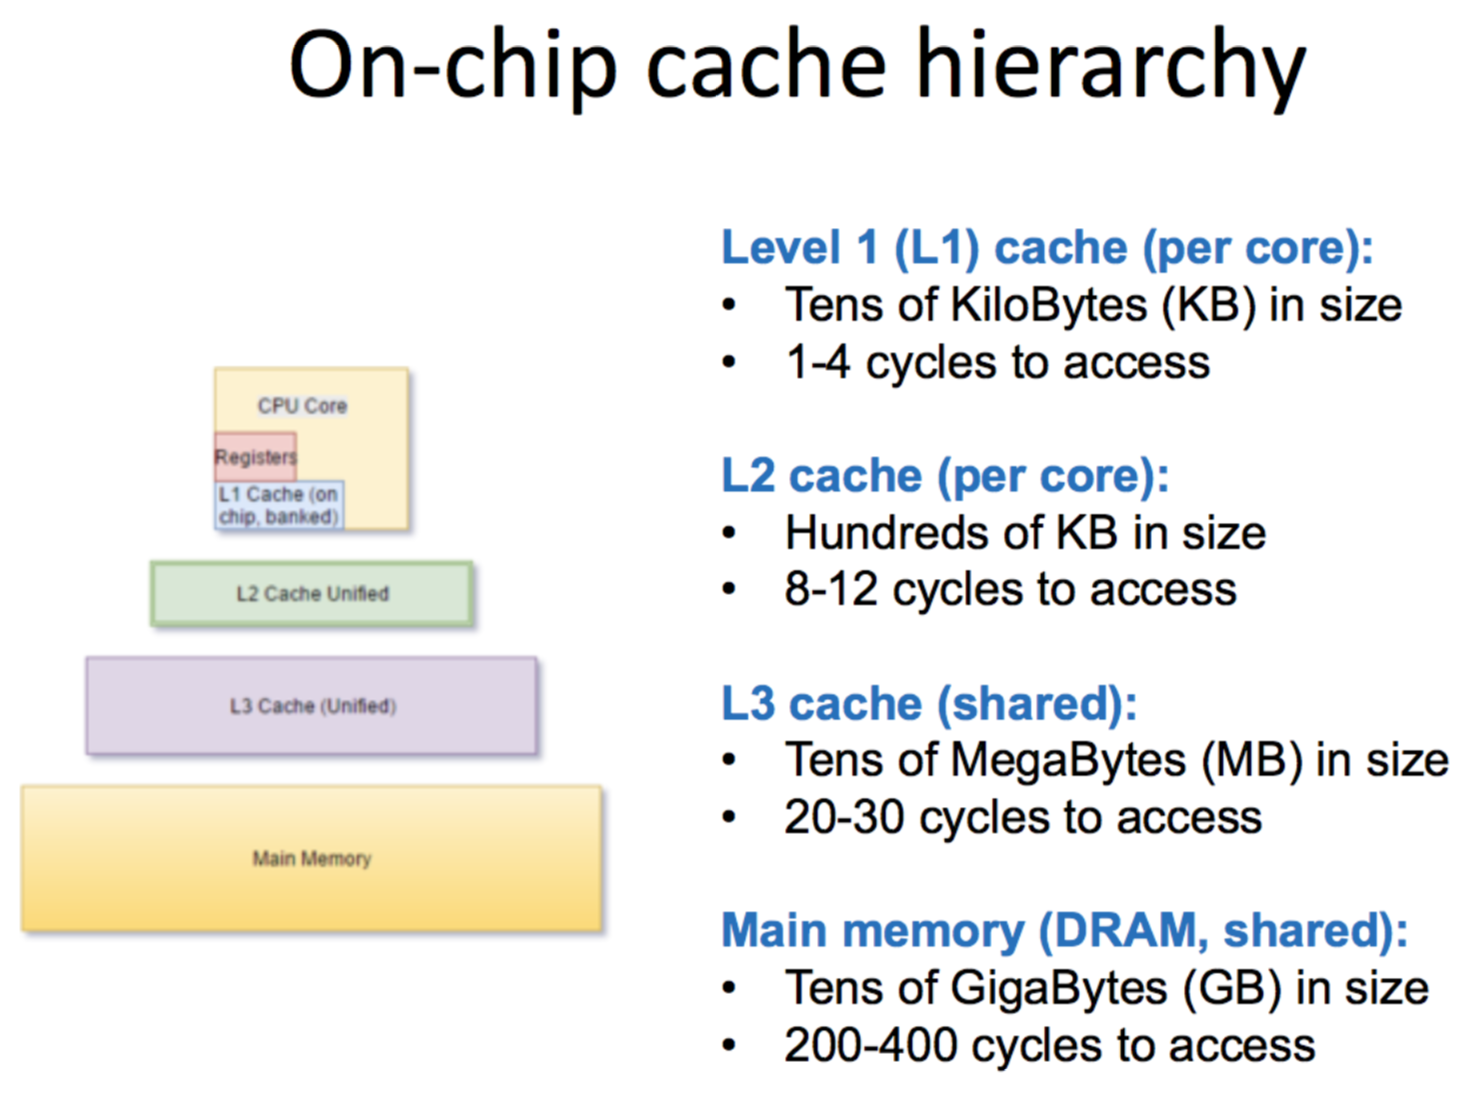
\includegraphics[scale=0.3]{images/cache-hierarchy.png}
    \caption{The Structure of Cache Hierarchy}
    \label{fig:my_label}
\end{figure}


\section{Serial Code Optimisations}

\begin{itemize}
    \item Algorithm Matter: different algorithms have different complex rate.
    \item Examine the within-core performance: finding the critical code and only attempting to optimise the critical code.
    \item Compiler and Flags:
    \begin{itemize}
        \item \href{https://gcc.gnu.org/onlinedocs/gcc/index.html}{\textcolor{blue}{gcc}} flags: -O2, -O3, -ffast-math
        \item \href{http://scv.bu.edu/computation/bladecenter/manpages/icc.html}{\textcolor{blue}{icc}} flags: -fast
    \end{itemize}
    \item The memory hierarchy:
    \begin{itemize}
        \item Row vs. Column Major Order
        \item don’t re-visit memory
        \item 'Blocked' loop
    \end{itemize}
    \item Vectorisation: making use of wide registers is important on modern processors (\href{https://software.intel.com/sites/landingpage/IntrinsicsGuide/}{\textcolor{blue}{SIMD}}: SSE, AVX, AVX2, AVX512).
\end{itemize}


\section{OpenMP}

OpenMP (Open Multi-Processing) is an application programming interface (API) that supports multi-platform shared memory multiprocessing programming in C, C++ and Fortran on most platforms.

\textbf{Threads vs. Processes}: Multiple threads can exist within the same process and share resources such as memory, while different processes do not share these resources.

\textbf{Two Method for Multi-threads}:

\begin{itemize}
    \item The old way: \href{https://computing.llnl.gov/tutorials/pthreads/}{\textcolor{blue}{Posix Threads}}, it is tedious and error prone.
    \item \href{http://www.openmp.org/}{\textcolor{blue}{OpenMP}}: serial code with \textit{\#pragma} compiler directives.
\end{itemize}

\begin{figure}[h]
    \centering
    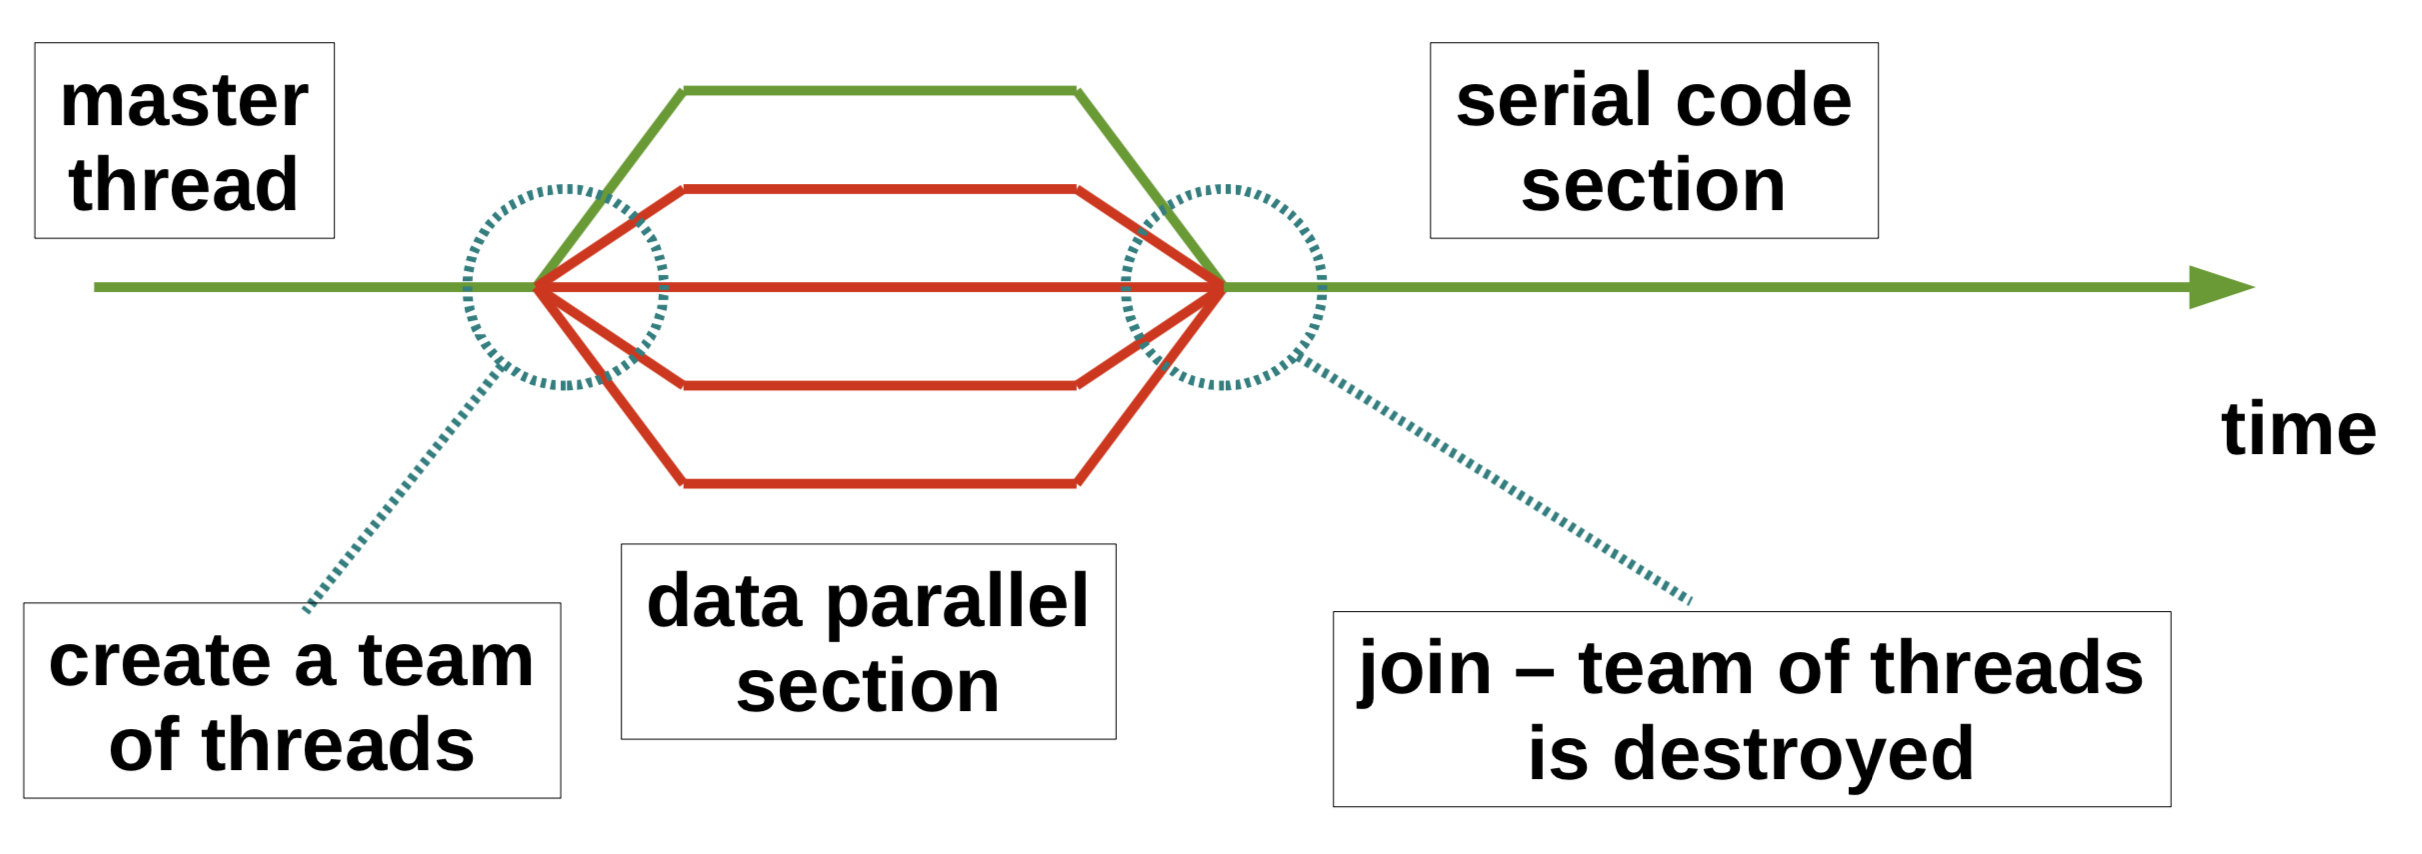
\includegraphics[scale=0.2]{images/openmp.png}
    \caption{Open MP}
    \label{fig:my_label}
\end{figure}

\subsection{Key Features}

\begin{itemize}
    \item Compiler directives: \textit{\#pragma}
    \item Thread team creation: \textit{parallel}
    \item Data attributes: \textit{shared}, \textit{private}
    \item Team operations: \textit{reduction}
    \item Work sharing: \textit{for} in loops; \textit{section}, \textit{task} in less structured.
    \item Syncronisation:
    \begin{itemize}
        \item Implicit at end of work sharing loops
        \item Mutex (one processor at a time): \textit{critical}
        \item Wait for all threads: \textit{barrier}
        \item One thread executes: \textit{single}, \textit{master}
    \end{itemize}
\end{itemize}

\subsection{Runtime Library}

\begin{itemize}
    \item Get the number of threads in team: \textit{omp\_get\_num\_threads()}
    \item Get the thread id: \textit{omp\_get\_thread\_num()}
    \item Control the number of threads via an environment var: \textit{OMP\_NUM\_THREADS}
    \item Control the number in the program: \textit{omp\_set\_num\_threads(N)}
\end{itemize}


\subsection{Performance}

\textbf{Accumulator}

\begin{itemize}
    \item Shared Accumulator lead to a long critical bocking time.
    \item Array of Accumulators leads to thrashing cache.
    \item Private Accumulators.
    \item Reduction will make a copy of the reduction variable per thread, and after the loop, the local variable will be combined into the global variable using the reduction operator.
\end{itemize}

\textbf{Schedule}

\begin{itemize}
    \item \textit{static}: dividing the loop into equal-sized chunks or as equal as possible.
    \item \textit{dynamic}: using a work queue to give a chunk- sized block of tasks to each thread.
    \item \textit{guided}: same to dynamic scheduling, but the chunk size is decreasing.
\end{itemize}

\textbf{The \textit{nowait} Clause} allows program to avoid the implicit barrier at the end of a worksharing for loop.

\subsection{Potential Benefits}

\textbf{Amdahl's Law}

\begin{equation}
    speedup = \frac{T_1}{T_p}
\end{equation}
\begin{equation}
    speedup_{max} = \frac{1}{1-P}
\end{equation}
\begin{equation}
    speedup_{ideal} = \frac{1}{\frac{P}{N} + S}
\end{equation}

Notice that:
\begin{itemize}
    \item $T_1$ is the execution time on a single processor.
    \item $T_p$ is the execution time on a parallel computer.
    \item $S$ is the serial fraction of the program.
    \item $P$ is the parallelisable fraction of the program.
    \item $N$ is the number of processors available.
\end{itemize}

\textbf{Gustafson's Law}

\begin{equation}
    speedup = \frac{T_1}{T_p} = \frac{T_{a}(x) + N \times T_{b}(x)}{T_{a}(x) + T_{b}(x)} \rightarrow N
\end{equation}

Notice that:
\begin{itemize}
    \item $x$ is a measure of problem size.
    \item $N$ is the number of processors.
    \item $T_a(x)$ is fraction of time spent executing the serial part of the program.
    \item $T_b(x)$ is fraction of time spent executing the parallel part.
\end{itemize}


\subsection{New features in OpenMP v4}

\textbf{NUMA}: Under NUMA, a processor can access its own local memory faster than non-local memory, which also provides higher overall memory bandwidth. It uses 'first touch' policy to control placement of items across the banks of memory.


\begin{figure}[h]
    \centering
    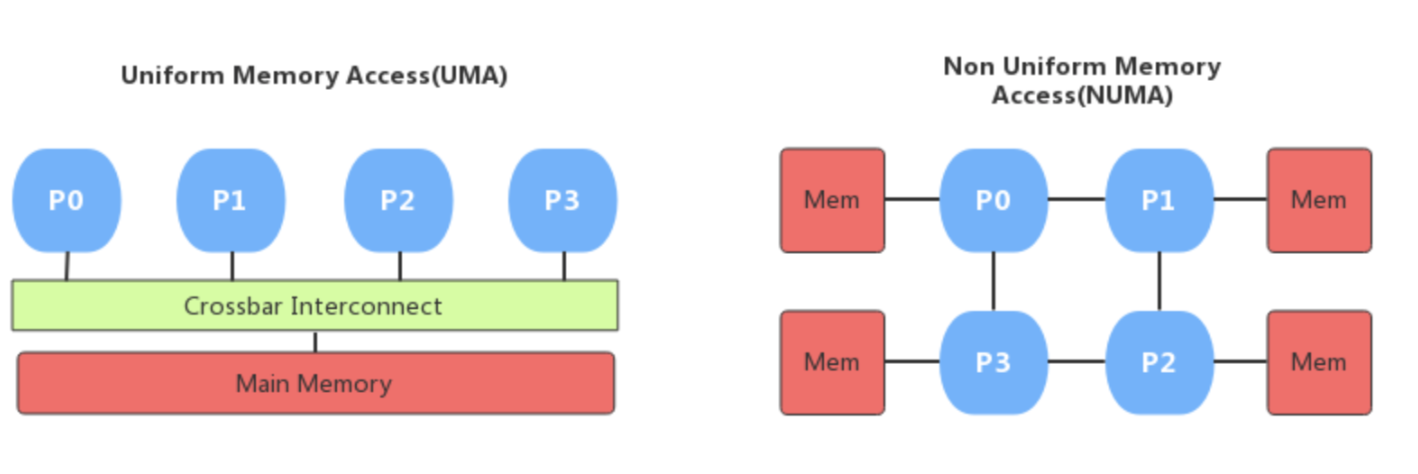
\includegraphics[scale=0.4]{images/uma-numa.png}
    \caption{UMA vs. NUMA}
    \label{fig:my_label}
\end{figure}

\textit{binding policy}:
\begin{itemize}
    \item threads: corresponding to a single hardware thread. \item cores: corresponding to a single core.
    \item sockets: corresponding to a single socket.
\end{itemize}

\textbf{SIMD Directive}: a work sharing loop can be executed using SIMD lanes \textit{\#pragma omp parallel for simd}.


\section{Roofline Model}

The Roofline model is an intuitive visual performance model used to provide performance estimates of a given compute kernel or application running on multi-core, many-core, or accelerator processor architectures, by showing inherent hardware limitations, and potential benefit and priority of optimizations.

Operational Intensity:

\begin{itemize}
    \item Operations per byte of memory traffic.
    \item An operation could be floating point, integer... Traffic is measured at main memory (DRAM).
\end{itemize}

\begin{equation}
    OI = (ops)/(bytes).
\end{equation}

\begin{multline}
Attainable\ GFLOP /s = \\
min \left\{\begin{matrix} Peak\ floating - point\ per\ formance \\ Peak\ memory\ bandwidth * Operational\ intensity \end{matrix}\right.
\end{multline}

\begin{figure}[h]
    \centering
    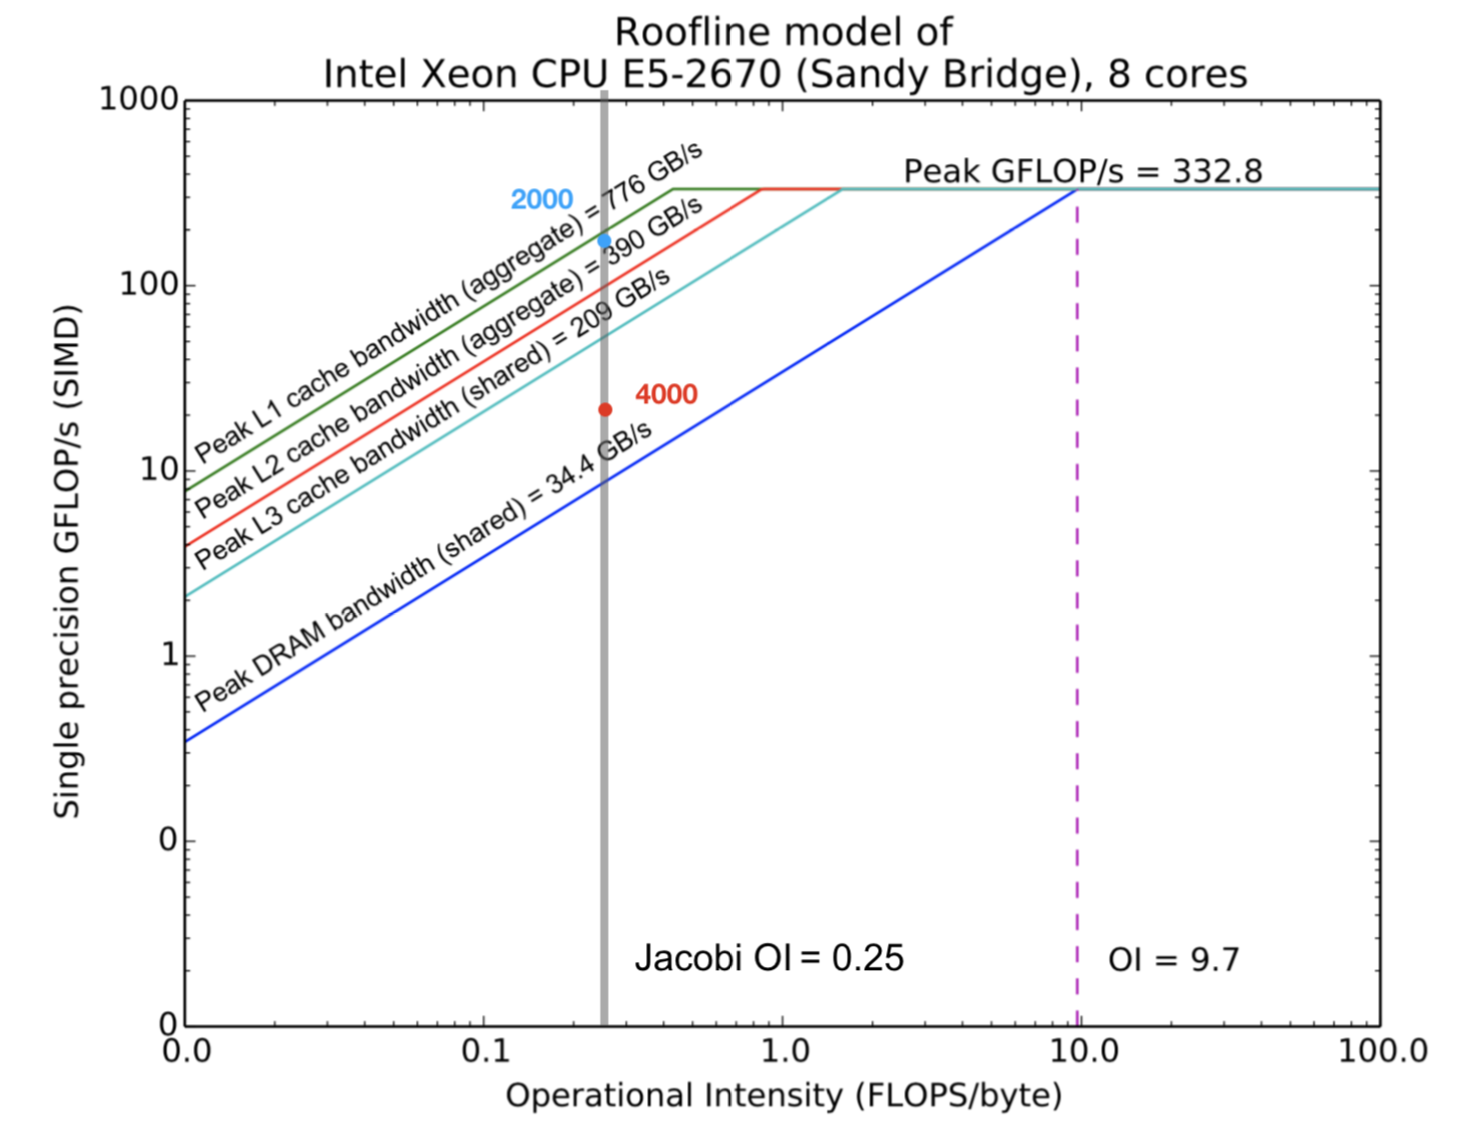
\includegraphics[scale=0.5]{images/roofline-model.png}
    \caption{The Example of Roofline Model}
    \label{fig:my_label}
\end{figure}

\section{OpenMPI}

The Open MPI Project is an open source Message Passing Interface implementation that is developed and maintained by a consortium of academic, research, and industry partners. MPI has a well-designed library that is intended to be portable and it is available for C and Fortran.


Point-to-point communication




\begin{itemize}
    \item Asynchronous:
\begin{lstlisting}[language=C]
void MPI_Send(buffer, data_length, data_type,
        dest, tag, MPI_COMM_WORLD);
void MPI_Recv(buffer, data_length, data_type,
        source, tag, MPI_COMM_WORLD);
\end{lstlisting}

    \item Safe, Portable: \textit{MPI\_Ssend()}
    \item Buffered, Blocking send: \textit{MPI\_Bsend()}
    \item Non-blocking: \textit{MPI\_Isend()} and \textit{MPI\_Irecv()}
    \item Packed data messages: \textit{MPI\_Pack} and \textit{MPI\_unpack}
\end{itemize}


\end{document}
